%%%%%%%%%%%%%%%%%%%%%%%%%%%%%%%%%%%%%%%%%
% Weekly Report 
% LaTeX Template
% Version 1.3 (26/10/2018)
% Modified by
% Enes TAŞTAN
% Erdem TUNA
% Halil TEMURTAŞ
%%%%%%%%%%%%%%%%%%%%%%%%%%%%%%%%%%%%%%%%%
%
%----------------------------------------------------------------------------------------
%	PACKAGES AND OTHER DOCUMENT CONFIGURATIONS
%----------------------------------------------------------------------------------------
\documentclass[a4paper,12pt]{article}
%-----packages------
\usepackage[a4paper, total={6.2in, 8.5in}, headheight=110pt]{geometry}
\usepackage[english]{babel}
\usepackage[utf8x]{inputenc}
\usepackage{amsmath}
\usepackage{graphicx}
\usepackage[colorinlistoftodos]{todonotes}
\usepackage{gensymb} % this could be problem
\usepackage{float}
\usepackage{fancyref}
\usepackage{subcaption}
\usepackage[toc,page]{appendix} %appendix package
\usepackage{xcolor}
\usepackage{listings}


\usepackage[export]{adjustbox}

\usepackage{xspace}
\usepackage{amssymb}
\usepackage{nicefrac}
\usepackage{gensymb}
\usepackage{fancyhdr}
\usepackage{lipsum}  % for lipsum
\usepackage[final]{pdfpages}  % pdf include
\usepackage{array} %allows more options in tables
\usepackage{pgfplots,pgf,tikz} %coding plots in latex
\usepackage{capt-of} % allows caption outside the figure environment
\usepackage[export]{adjustbox} %more options for adjusting the images
\usepackage{multicol,multirow,slashbox} % allows tables like table1
%\usepackage[hyperfootnotes=false]{hyperref} % clickable references
\usepackage{epstopdf} % useful when matlab is involved
%\usepackage{placeins} % prevents the text after figure to go above figure with \FloatBarrier 
%\usepackage{listingsutf8,mcode} %import .m or any other code file mcode is for matlab highlighting

%-----end of packages
%\input{../../../Documents/configuration.tex}


\pagestyle{fancy}
\setlength\headheight{80pt}
\setlength{\footskip}{2.5cm}
%\fancyhead[LO,LE]{Duayenler Ltd. Şti.}
%\fancyhead[RO,RE]{October 19, 2018}
%\fancyhead[LO,LE]{\textbf{Duayenler Ltd. Şti.} \\ \textbf{Members :\\ } 
%			Enes Taştan, 2068989, 0543 683 4336 \\ 
%			Halil Temurtaş, 2094522, 0531 632 2194  		
%}
%\fancyhead[RO,RE]{
%			\textbf{XXXX, XX, 201X} \\
%			Sarper Sertel, 2094449, 0542 515 6039 \\
%			Erdem Tuna, 2167419, 0535 256 3320 \\ 
%			İlker Sağlık, 2094423, 0541 722 9573 		
%}
%\fancyhead[RO]{Sarper Sertel (05435156039),\\Enes Taştan (05436834336), Erdem Tuna (05352563320),\\Halil Temurtaş (05316322194), İlker Sağlık (05417229573)}

\begin{document}
	
\begin{center}
	\Large\textbf{24.11.2018 PDR+ Sunumu Feedback Raporu}
	\end{center}


\begin{itemize}

	\item Safetyci ve pilotla konuşulmalı
	
	\item TAI elektrik ve aviyonik mimari ile ilgili eğitimleri sağlayacak
	
	\item ICDC(sensörü olan her sistem için)
	
	\item İlerde wiring çizecek insan gücüne ihtiyaç olacak
	
	\item Her aviyoniğin giriş çıkışlarını/interfacelerini/subpartlarını ezbere bilen insanlar olmalı	
	
	

	\item Elektrik Mimari Güncellenecek
		\begin{itemize}
			\item Kim hangi bus a bağlanacak, büyük bi güncelleme gerekli
			\item Batarya/ Elektrik tesisat
			\item Jenarator/ Batarya bağlantısı
			\item Bataryanın ısınınca devreden çıkması lazım
			\item Aku state gosterilmesi laxim
			\item Generator olmayinca aku neye power verecek
			\item Şarj/ Disşarj olayları 
			\item Jenerator kaapanınca neler beslenecek
			\item Batarya ömrü 3 hafta sonra orjinal kapasitesinin 80\% ine düşecek. Hesaba kat
			\item Ekipmanlar çalışmaya başlarken anormal akım çekebiliyor (7*normal zaman akımı çeken telsiz örneği verildi) \textbf{[Demeraj akımı]}.
			\item Sistem Overload olmasın
			\item Ekipmanlarin ne sirayla start edilmesi bilinecek			
			\item Delayli başlama stratejisi benimsenmeli
			\item Motor alternatörü araştırma
			\item Batarya/Jenarator Gözlemi?
			\item Yeni Elektrik üretici gözleniyor mu?
			\item Diğer grupların ihtiyacını(actuator/servo vs kullanılan yerleri, tahmini requirementleri sorup[servo için kaç tok gerekiyor vs.]) assume edip, çalışmalara başlanmalı. Diğerlerini beklemek yerine onları elektrik konusunda dürtmek lazım
			\item Jenerator failure gosteriyor mu	
	
			
		\end{itemize}
	
	
	\item Aviyonik Mimarinin güncellenmesi ve sensörlerin yerleşimi/
		
	
		\begin{itemize}
			\item Telsiz/GPS ve diğer sensörlerin yerleşimi araştırılmalı		
			\newpage
			\item G5
				\begin{itemize}
					\item Gyro içinde mi?
					\item G5 PFL statüsünde mi (G500'e bağlamakla alakalı)
					\item G5 solo BFI mı olmalı
					\item G5 configured as aDG
					\item CVR/ FDR
					\item Solo olması için pitostatic portu var mı?
				\end{itemize}
			
			\item G500 TXI
				\begin{itemize}
					\item Pitostatic sensör seçimi/yerleşimi/ Garmin opsiyon mu?
					\item Tüpün bağlantısı/ geçeceği hat vs
					\item Tunahanların ekip ile iletişmen geçilmeli, pitotlarla ilgili
					 
				\end{itemize}
			
			\item GTN 750
				\begin{itemize}
					\item Nav dediğimiz ne tam olarak
					\item VOR? DME? IDC?
					\item \textbf{Telsizler Nerede?}
					\item Tek (sadece yer) mi çift(yer+diğer uçak) mi telsiz seçilecek
					\item Ekstra telsiz ile anten çoklayıcı ekipman devreye girecek(Elektik mimariye bir ek mesela)
					\item Anten seçimi
				\end{itemize}
			\item ELT Boyut
			
			\item GMA 345 ayrıntı
			
			\item GTX 345 ayrıntı
		\end{itemize}
		
	\item Kokpit güncelleme
		\begin{itemize}
			\item Uçuşlar genelde soldan yapılıyor, G500 10" sola,
			\item Önemli bilgiler ortada bulunmalı (hız, yükseklik, motor uyarı vs.). G500 7" ortaya
			\item G5 sensör dahili mi uzakta mı, dahiliyse şnterference için diğerlerinden uzakta bulunmalı 
			\item Kokpit grubunun çizimlerinde 7" lik ekranın boyutları 10" gibi çizilmiş, geri dönüş sağlanacak 
		\end{itemize}
	
	 \item Motor ile ilgili ek bilgiler istendi
	 
	 \item EIS için kullanılacak sensörler kısmen motor ve yakıt tankı içinde mevcut, kullanabiliyor muyuz ile ilgili diğer gruplarla iletişim kurulmalı (Motoru seçen grupla mesela)
	 
	 \item Bazı slayt sayfaları kullanışlı olabileceği düşünülerek eklendi. \textit{Figure~\ref{fig:fuel}} ve \textit{Figure~\ref{fig:gv}}.
	 
\begin{figure}[H]
\center
\setlength{\unitlength}{\textwidth} 
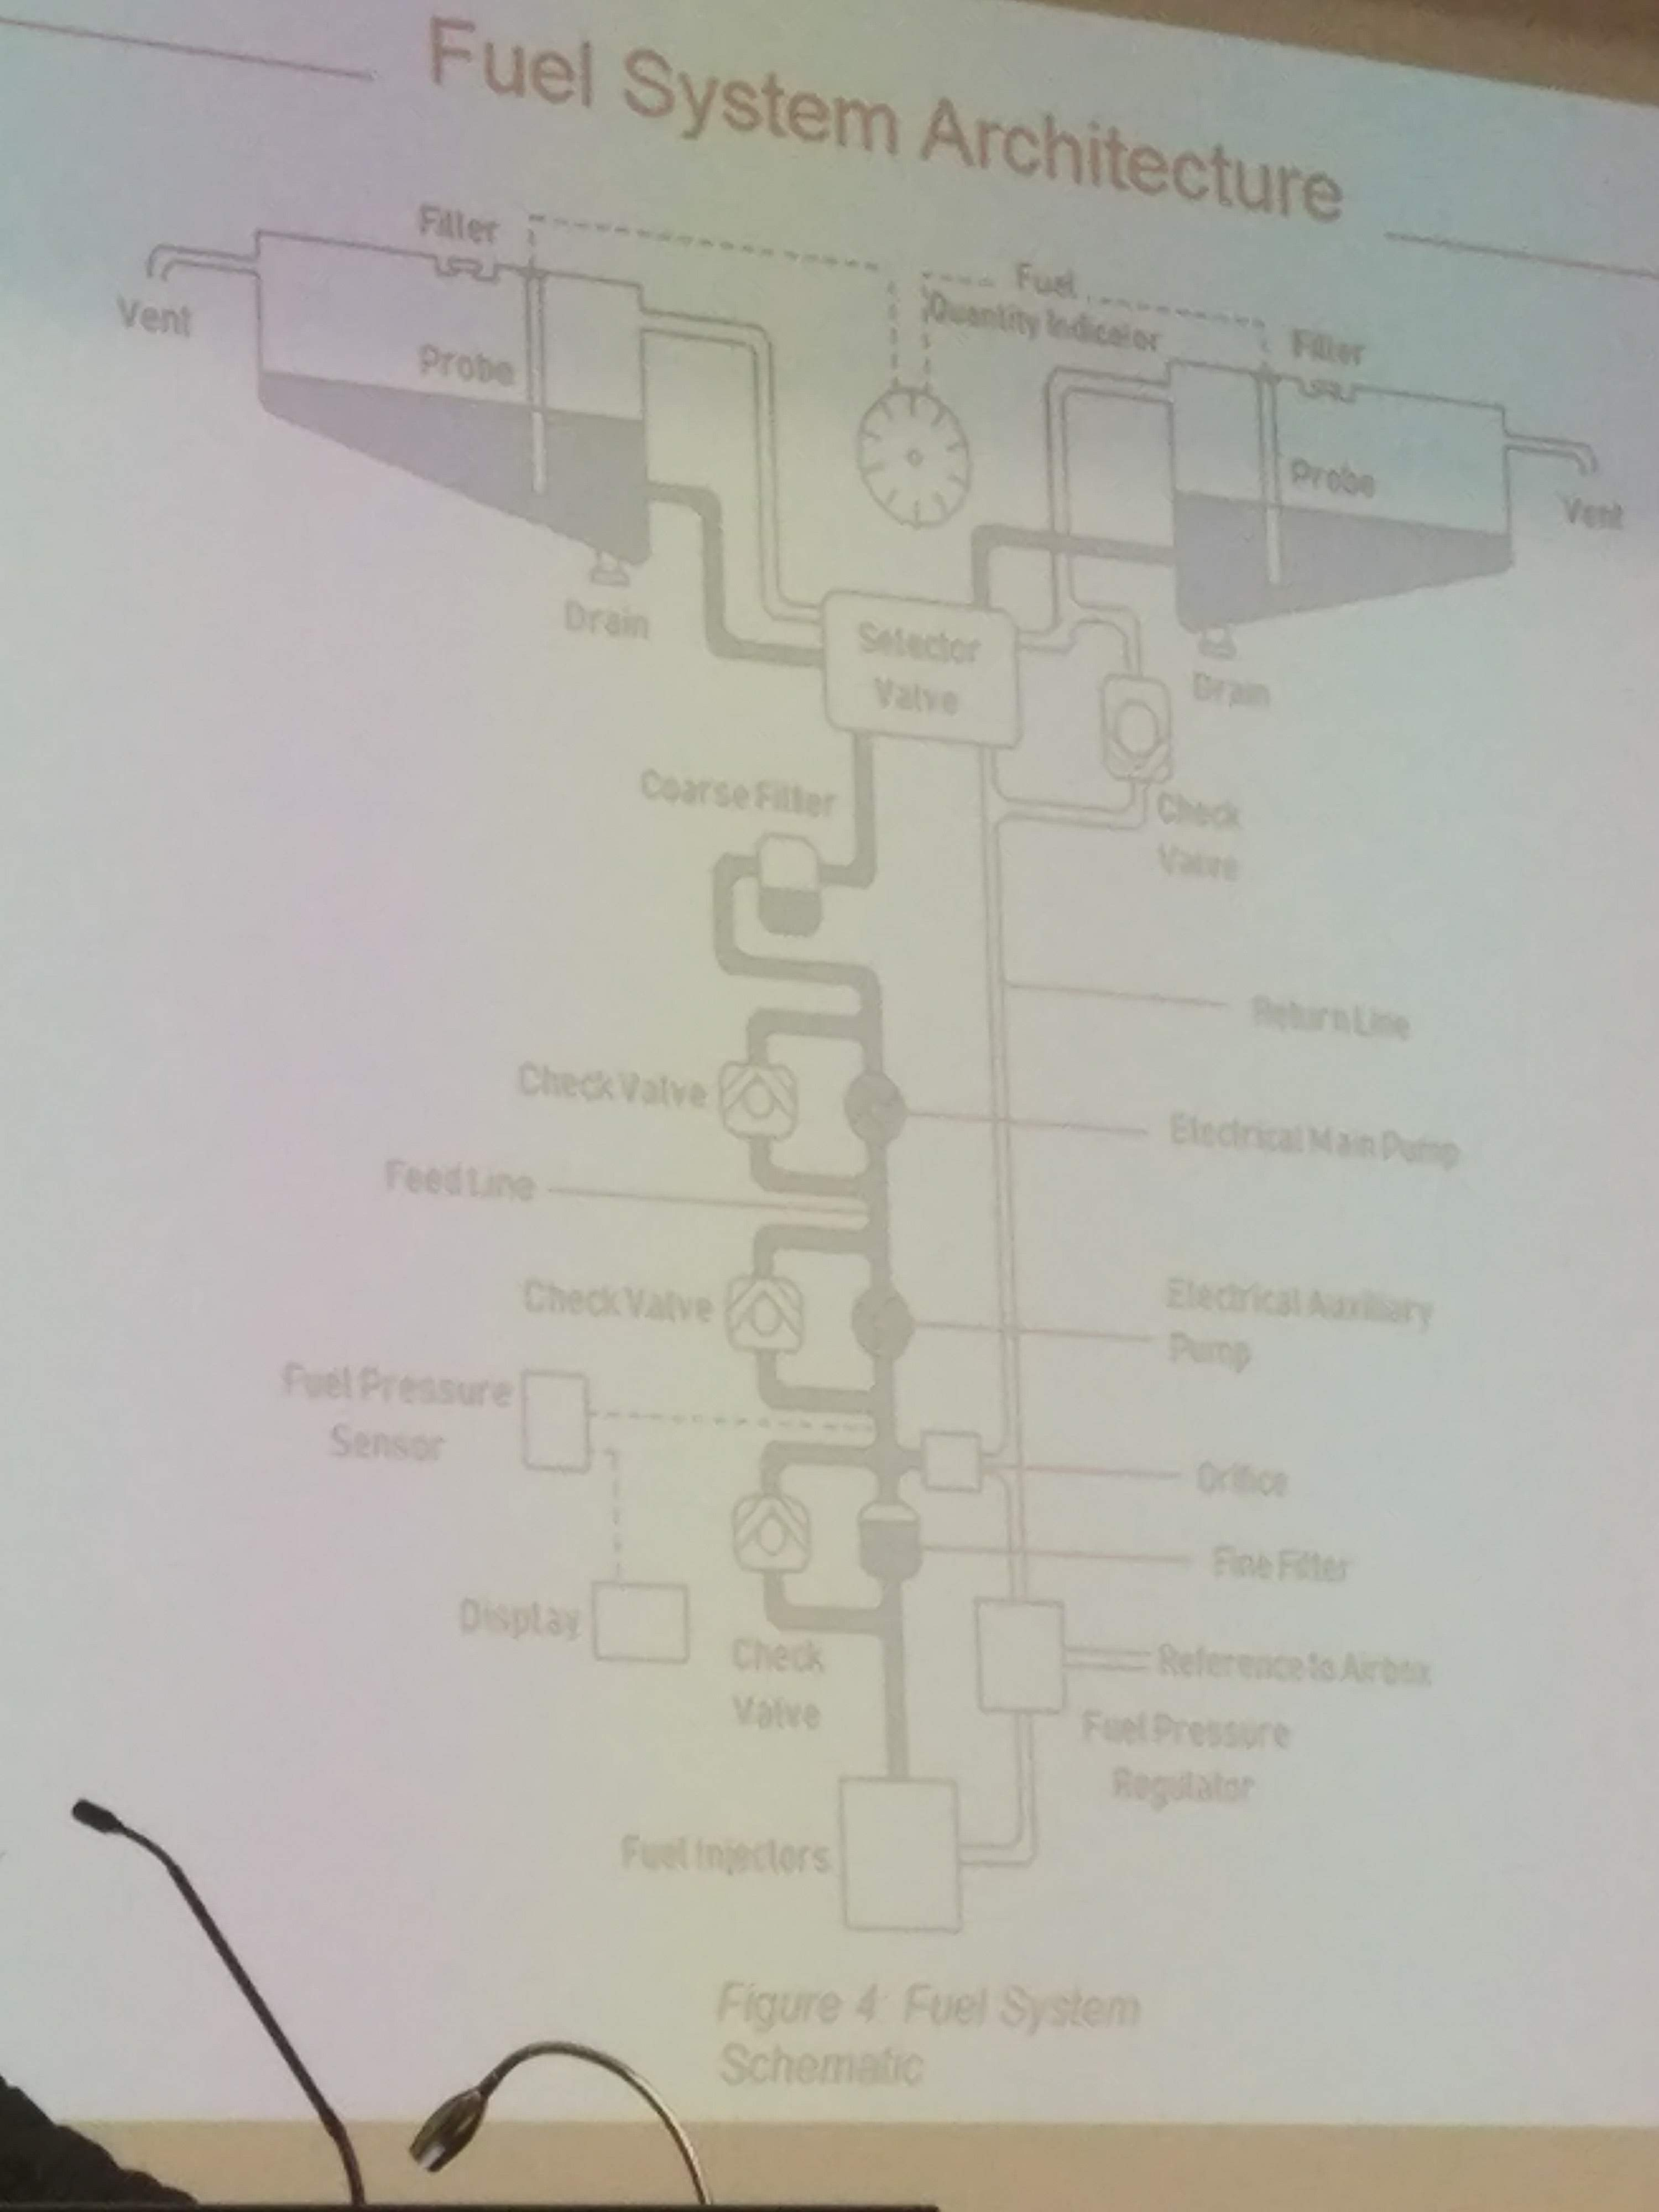
\includegraphics[width=0.9\unitlength]{1}
\caption{\label{fig:fuel} Fuel System Architecture }
\end{figure}
	
\begin{figure}[H]
\center
\setlength{\unitlength}{\textwidth} 
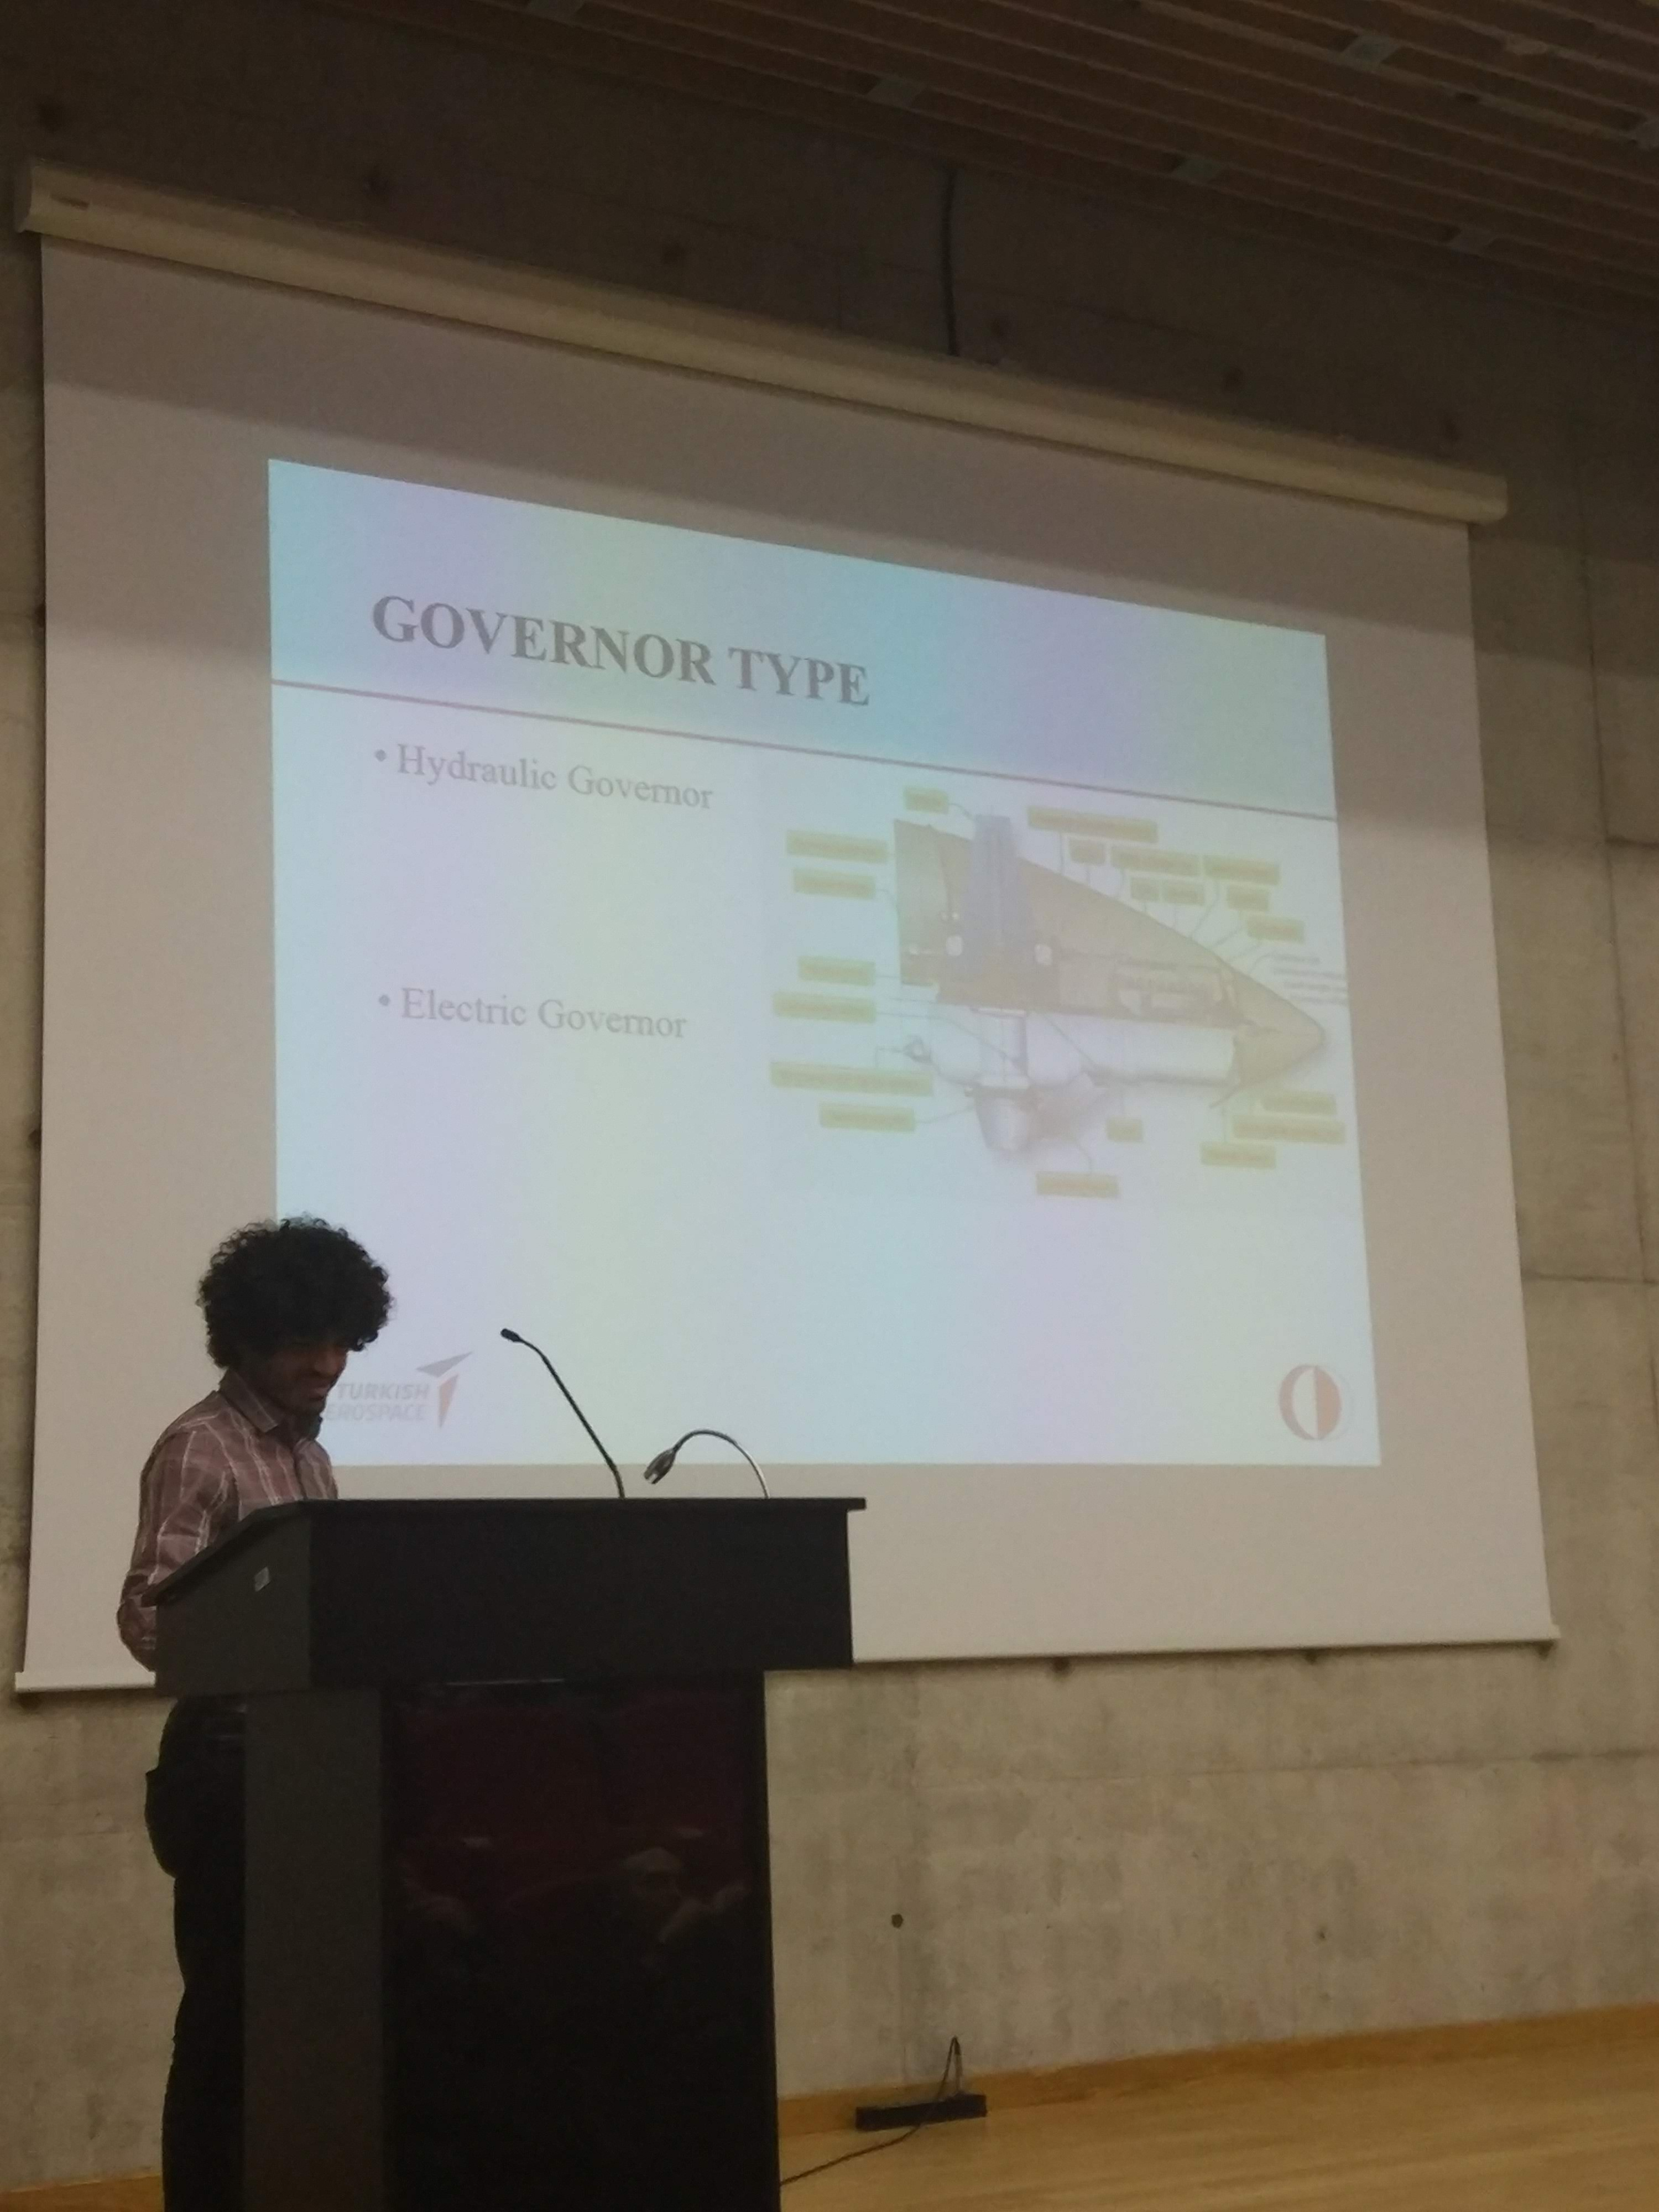
\includegraphics[width=1.0\unitlength]{2}
\caption{\label{fig:gv} Governor Types  }
\end{figure}
	
	
	
\end{itemize}



%\lipsum[1-5]

\end{document}

%----samples------
%\begin{itemize}
%\item Item
%\item Item
%\end{itemize}

%\begin{figure}[H]
%\center
%\setlength{\unitlength}{\textwidth} 
%\includegraphics[width=0.7\unitlength]{images/logo1}
%\caption{\label{fig:logo}Logo }
%\end{figure}

%\begin{figure}[H]
%	\setlength{\unitlength}{\textwidth} 
%	\centering
%	\begin{subfigure}{.5\textwidth}
%  		\centering
%  		\includegraphics[width=0.48\unitlength]{images/logo1}
%  		\caption{\label{fig:logo1}Logo1 }
%	\end{subfigure}%
%	\begin{subfigure}{.5\textwidth}
%  		\centering
%		\includegraphics[width=0.48\unitlength]{images/logo2}
%  		\caption{\label{fig:logo2}Logo2}
%	\end{subfigure}
%\caption{\label{fig:calisandegree} Small Logos   }
%\end{figure}
	
%\begin{table}[H]
%  \centering
% 
%    \begin{tabular}{c|c|c}
%       $$A$$ & $$B$$ & $$C$$ \\ \hline
%       1 & 2 & 3  \\ \hline
%       2 & 3 & 4  \\ \hline
%       3 & 4 & 5  \\ \hline
%       4 & 5 & 6  
%      
%  \end{tabular}
%  \caption{table}
%  \label{tab:table}
%\end{table}
	
%\begin{table}[H]
%  \centering
% 
%    \begin{tabular}{c|c|c}
%       \backslashbox{$A$}{$a$} & $$\specialcell{ Average deviation \\ after subtracting out the  \\ frequency error }$$ & $$C$$ \\ \hline
%       \multirow{2}{*}{1} & 2 & 3  \\ \cline{2-3}
%        & 3 & 4  \\ \hline
%       3 & \multicolumn{2}{c}{4}  \\ \hline
%       4 & 5 & 6  
%      
%  \end{tabular}
%  \caption{table}
%  \label{tab:table}
%\end{table}
%-----end of samples-----